\documentclass[12pt, french]{article}

\usepackage{fancyhdr, fancybox, lastpage}
\usepackage[most]{tcolorbox}
\usepackage[a4paper, margin={0.3in, .75in}]{geometry}
\usepackage{wrapfig}
\pagestyle{fancy}
\renewcommand\headrulewidth{1pt}
\renewcommand\footrulewidth{1pt}
\fancyhf{}
\rhead{ \em{Zakaria Haouzan}}
\lhead[C]{\em{Tronc Commun scientifique - option français (TCSBiof)}}
\chead[C]{}
\rfoot[C]{}
\lfoot[R]{}
\cfoot[]{\em{Page \thepage / \pageref{LastPage}}}


\newtcolorbox{Box2}[2][
enhanced, 
    breakable,
]{
                lower separated=false,
                colback=white,
colframe=white!20!black,fonttitle=\bfseries,
colbacktitle=white!30!gray,
coltitle=black,
enhanced,
attach boxed title to top left={yshift=-0.1in,xshift=0.15in},
title=#2,#1}


\begin{document}
\begin{center}
   \shadowbox {\bf{La tension électrique }}
\end{center}
\begin{center}
   \Large{ \em{Exercices Supplémentaires}}
\end{center}

%%_________________________Exercice ! :"_________________________Exercice
   \begin{Box2}{Exercice 1 : loi des mailles }

\begin{wrapfigure}[2]{r}{0.22\textwidth}

	\vspace{-0.8cm}
  \begin{center}
	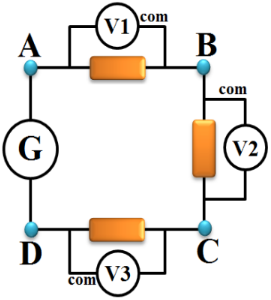
\includegraphics[width=0.22\textwidth]{./img/ex00.png}
  \end{center}
\end{wrapfigure}

	On considère le circuit du schéma ci-contre:
	\begin{enumerate}

		\item Pour chacun des voltmètres du schéma ci-contre, indiquer le nom de la
tension mesurée, en fonction des noms des points placés sur le circuit.
\item  Représenter chacune de ces tensions par une flèche.

\item Les valeurs mesurées sont : voltmètre $V_1= 2,5V$; voltmètre $V_2= -3,1V$; voltmètre $V_3= 6,4V$.
	\begin{enumerate}
		\item En appliquant la loi des mailles à ce circuit (indiquer le sens de
		parcours), déterminer la valeur de la tension $U_{AD}$. Quelle est la borne
positive du générateur?

\item  Ecrire $U_{AD}$ en fonction de $U_{AB}$, $U_{BC}$ et $U_{CD}$. Montrer que cette relation
	permet de retrouver la même valeur de $U_{AD}$.
		

\end{enumerate}
	\end{enumerate}
   \end{Box2}


%%_________________________Exercice !2 :"_________________________Exercice
\begin{Box2}{Exercice 2 :courant et tension}

	\begin{wrapfigure}[2]{r}{0.4\textwidth}
  \begin{center}
	  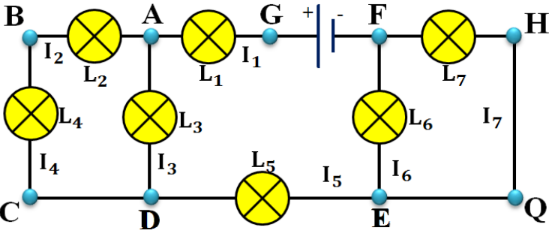
\includegraphics[width=0.4\textwidth]{./img/ex01.png}
  \end{center}
\end{wrapfigure}
Soit le circuit représenté ci-dessous. Il
comporte un générateur et plusieurs lampes.
Seules les lampes (L6) et (L7) sont identiques.



	\begin{enumerate}
		\item Indiquer le sens du courant dans chaque
branche \\du circuit.
\item  Comparer, en justifiant votre réponse, les
valeurs \\de $I_2$ et $I_4$.
\item  Ecrire la loi des nœuds au nœud A. En déduire la valeur de $I_3$.
\item Indiquer sur le schéma du circuit l’emplacement de l’ampèremètre pour mesurer l’intensité $I_3$.
\item  Calculer $I_5$, $I_6$ et $I_7$.
\item  Représenter les tensions $U_{AB}$ et $U_{CB}$.
\item  Quelle est la valeur de la tension $U_{CD}$ ? Justifier.
\item  Ecrire la loi des mailles dans la maille ABCDA. Et calculer la tension $U_{AD}$ et déduire $U_{GA}$.
\item  Représenter sur le schéma du circuit, le branchement du voltmètre pour mesurer la tension $U_{GA}$.
\item Comparer, en justifiant votre réponse, les tensions $U_{EF}$ et $U_{HF}$.
\item Déterminer les valeurs des tensions $U_{EF}$ et $U_{HF}$.
\end{enumerate}

Données: $I_1 = 0,1A$; $I_4 = 20 mA$; $U_{AB} = 4 V$; $U_{CB} = - 2 V$; $U_{GD} = 7 V$; $U_{ED} = - 1 V$ et $U_{GF} = 10 V$.


\end{Box2}

%%%_________________________Exercice ! 3:"_________________________Exercice
%\begin{Box2}{Exercice 3 :intensité du courant  }
   %% \begin{wrapfigure}[2]{r}{0.25\textwidth}
  %%\begin{center}
	%%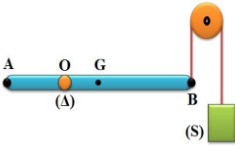
\includegraphics[width=0.25\textwidth]{./img/ex02.png}
  %%\end{center}
%%\end{wrapfigure}
%\begin{enumerate}
%\item Sur quelle graduation se fixera l'aiguille de l'ampèremètre?
%\end{enumerate}
%\end{Box2}





%%%_________________________Exercice 4 : _________________________Exercice
%\begin{Box2}{Exercice 4 :Utilisation d'un ampèremètre }

	%%\begin{wrapfigure}[1]{r}{0.28\textwidth}
		%%\vspace{-0.5cm}
  %%\begin{center}
	%%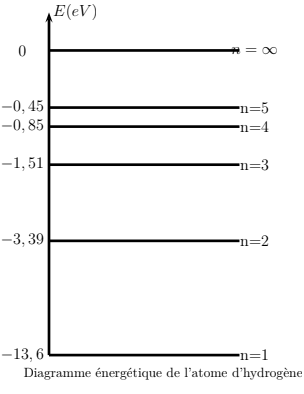
\includegraphics[width=0.28\textwidth]{./img/ex04.png}
  %%\end{center}
%%\end{wrapfigure}
%\begin{enumerate}
	%\item 2
%\end{enumerate}
%\end{Box2}


%%%_________________________Exercice 5 : _________________________Exercice
%\begin{Box2}{Exercice 5 :application de la loi des nœuds  }
   %% \begin{wrapfigure}{r}{0.25\textwidth}
  %%\end{wrapfigure}
%\end{Box2}
%%%%_________________________Exercice 6 : _________________________Exercice

%\begin{Box2}{Exercice 6 :Exploitation des circuits électriques}
%\end{Box2}


%\begin{Box2}{Exercice 7 : Influence d'un dipôle sur la valeur de l'intensité du courant  }

%\end{Box2}



%\begin{Box2}{Exercice 8 : Synthèse  }
%\end{Box2}


%\begin{Box2}{Exercice 9 : Synthèse  }



%\end{Box2}



\begin{center}
	\emph{If it weren't for electricity, we'd all be watching television by candlelight.}

	\emph{\textbf{Future Is Loading...}}

\end{center}

\end{document}
